\documentclass{report}

\usepackage[top=2cm, left=2cm, right=2cm, bottom=2cm]{geometry}
\usepackage{amsmath}
\usepackage{amsfonts}
\usepackage{mdframed}
\usepackage{tikz}
\usepackage{graphicx}
\usepackage{subfig}
\usetikzlibrary{arrows}
\usetikzlibrary{decorations.pathmorphing}
\usetikzlibrary{shapes}

\newcommand\WLOG{{\small\textbf{WLOG}}}

\title{Data analysis and data Mining\\Report 2}

\author{Mauro Angelini\\
Alessio Gilardi}

\begin{document}
    \maketitle
    \tableofcontents

    \setlength\parskip{0.5cm}
    
	\chapter*{First exercise}
	\addcontentsline{toc}{chapter}{First exercise}
	
We define a multiclass classification problem.\\
Being a multiclass problem it is necessary to use a one-vs-all or all-vs-all method.
In this case we use a linear classifier with an all-vs-all method, in which each class is compared to all the others with each new iteration of the algorithm.\\
We use a $\lambda$ as regularization parameter.
To get the best solution we divide the dataset into two sets: a learning set, corresponding to the $ 70 \% $ of the initial data and a validation set, in order to calculate the error committed by our model, and run a loop on different $\lambda$ values in order to identify the best value.\\
To mediate the result and minimize the influence of variance we repeat this procedure a number k of times, with k equal to 30 for example.
\begin{figure}[h]
	\centering
	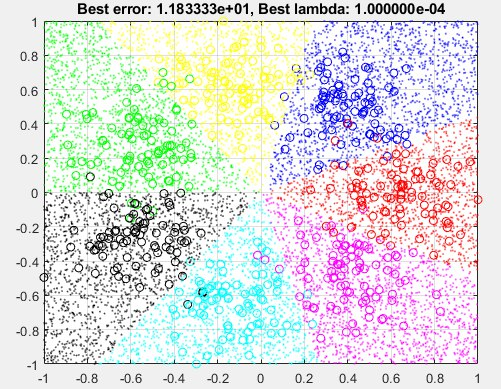
\includegraphics[width=0.5\textwidth]{i1.png}
	\caption{Regression Function}
	\label{fig:regression function}
\end{figure}


 
	
	\setlength\parskip{0.5cm}
	
    \chapter*{Second exercise}
    \addcontentsline{toc}{chapter}{Second exercise}
    	
We define another classification problem that we treat this time with $SVM $.	
In this scenario the parameter to be optimized is C: this parameter can be interpreted as the inverse of $\lambda$, so for small $C$ we will have a smoother solution, while for big $C$ we will only worry about minimizing the mistake.
To do this, as usual, we divide the dataset into two parts: Training Set and Validation Set and execute a cycle on the variable C, memorizing the error defined as the number of wrong classifications. To minimize the variance we repeat the procedure k times.
Once this is done, we look for the error with the lowest number of wrong classifications in the error vector, the corresponding $C$ will be $C_{best}$.	
We repeat, at this point, the calculation performed before using $C_{best}$ instead of $ C $ and plotting the solution.
In the two graphs below we show two cases: in the first, with the same error, we choose the $C_{best}$ lower, so the solution will be smoother, but less precise: there will be many points with $ 0 <\alpha_i<=C$ (we will have a $\underline{w}$ low), while in the second one, with the same error we favor greater $C_{best}$, so the solution will be more complex, but with $\alpha$ vector more sparse.	
\begin{figure}[!ht]
	\centering
	\subfloat[][\emph{Smaller C}.]
	{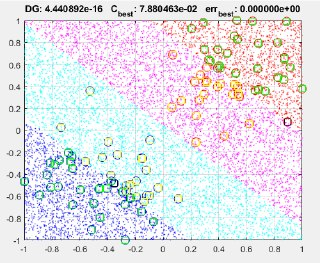
\includegraphics[width=0.4\textwidth]{i6.png}} \quad
	\subfloat[][\emph{Greater C}.]
	{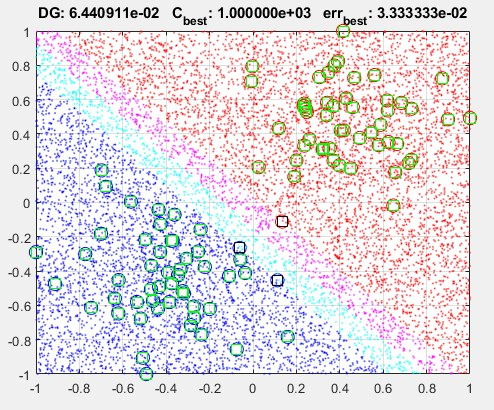
\includegraphics[width=0.4\textwidth]{i7.png}} \\
	
\end{figure}

	
	\setlength\parskip{0.5cm}
	
	\chapter*{Third exercise}
	\addcontentsline{toc}{chapter}{Third exercise}
	
In this exercise we implement a multiclass classification problem with a Decision Tree.
We start from the binary case and extend it to the multiclass problem.\\
The parameter to be optimized in this problem can be the depth of the tree.\\
Also in this case we divide the dataset into two sets, the learning set and the validation set and using the validation set we calculate the error as the number of points classified incorrectly. Here again we repeat the product k times, with k equal to 30.\\

\begin{figure}[h]
\centering
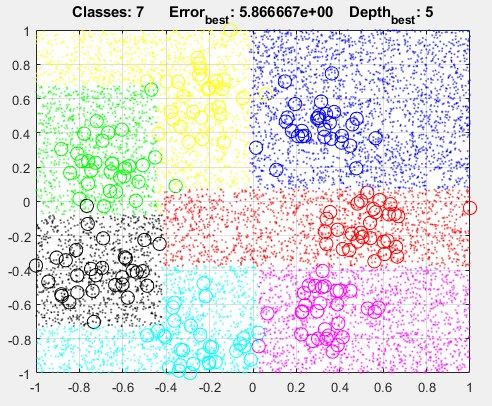
\includegraphics[width=0.5\textwidth]{i3.png}
\caption{Regression Function}
\label{fig:regression function}
\end{figure}
\begin{figure}[h]
Finally, we took a dataset with 3 features, in order to be plottable in 3D, and 3 classes. 
As before we divided dataset in training set and validation set, we used $ 70\%$ of data in training and the remaining for validation. Then we ran a loop on k and on depth to optimize the depth parameter.\\ \\ \\ \\


	\centering
	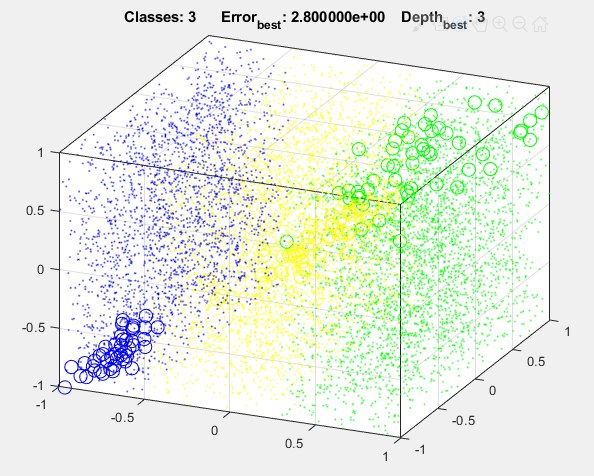
\includegraphics[width=1\textwidth]{i4.png}
	\caption{Regression Function}
	\label{fig:regression function}
\end{figure}

	
	\setlength\parskip{0.5cm}
	
 
    \listoffigures

\end{document}